\documentclass[output=paper,hidelinks]{langscibook}
\ChapterDOI{10.5281/zenodo.13347662}
\author{Christine Elsweiler\affiliation{LMU Munich} and Judith Huber\affiliation{Friedrich-Alexander-Universität Erlangen-Nürnberg}}
\title[Loss of number in the English 2nd person pronoun]{Loss of number in the English 2nd person pronoun: A change for the worse, but due to a change for the better?}  
\abstract{The article approaches recognized changes in the paradigm of the 2nd person personal pronoun as changes ``for the worse" or ``for the better". The loss of the 2nd person singular pronoun \textit{thou/thee} by the eighteenth century left standard English with \textit{you} as the only address pronoun, with no distinction in number anymore. We argue that the emergence of new forms such as \textit{you guys, y’all, youse, yinz}, which re-establish the number distinction, indicates that this was a ``change for the worse" for speakers. Can this change, however, also be viewed as a by-product of a change for the better on another level? We discuss two possible changes for the better involved in the loss of number of the 2nd person: (a) before \textit{thou/thee} was lost in Standard English, a two-term address pronoun system had developed, which offered speakers a means of pragmatic differentiation. (b) the loss of the \textsc{2sg} verbal ending \{\textit{-st}\}, which disappears together with \textit{thou}, can be considered as a change for the better in the verbal inflectional system.}

\IfFileExists{../localcommands.tex}{
  \addbibresource{../localbibliography.bib}
  \usepackage{tabularx,multicol}
\usepackage{url}
\urlstyle{same}

\usepackage{listings}
\lstset{basicstyle=\ttfamily,tabsize=2,breaklines=true}

\usepackage{langsci-optional}
\usepackage{langsci-lgr}
\usepackage{langsci-gb4e}
% \usepackage{langsci-textipa}

\usepackage{csquotes}
\usepackage{multirow}
\usepackage{colortbl}
\usepackage{ulem}
\usepackage{graphicx}
\usepackage{amsmath}
\usepackage{nicefrac}
\usepackage{tabto}
\usepackage{subcaption}
\usepackage{enumitem}
\usepackage{subcaption}


\usepackage{siunitx}
\sisetup{detect-weight=true, detect-family=true, detect-all, input-symbols={\%}, free-standing-units,group-digits=false,detect-inline-weight=math}

\usepackage[linguistics, edges]{forest}
\usetikzlibrary{matrix, arrows, arrows.meta}

\usepackage{pgfplots}
\usepgfplotslibrary{colorbrewer}
\pgfplotsset{cycle list/Dark2-4}

\usepackage{derivative}
\usepackage{langsci-branding}

  
\AtBeginDocument{%
  \SetupAffiliations{output in groups = false, 
                     separator between two = {\bigskip\\},
                     separator between multiple = {\bigskip\\},
                     separator between final two = {\bigskip\\}
                   }%
}

\newfontfamily\cjkfont
  [Scale=MatchLowercase]{SourceHanSerifSC-Regular.otf}
\AdditionalFontImprint{Source Han Serif}

\newcommand{\SC}{S\=uzh\=ou Chinese}
\newcommand{\MC}{Standard Chinese}
\newcommand{\THW}{T\`{a}ih\'{u} W\'{u}}
\newcommand{\SH}{Sh\`{a}ngh\v{a}i}
\newcommand{\iz}{ɨ̻}
\newcommand{\yz}{ʉ̻}
\newcommand{\zz}{ɿ}
\newcommand{\zw}{ʮ}
\newcommand{\pri}{*\textit{i}}
\newcommand{\pry}{*\textit{y}}
\newcommand{\prien}{*\textit{jen}}
\newcommand{\pryen}{*\textit{ɥɤn}}

\newcommand{\spr}[1]{\textsuperscript{#1}}

\renewcommand{\NG}{ŋ}
\newcommand{\textsubarch}{̯}
\renewcommand{\textschwa}{ə}
\renewcommand{\textprimstress}{ˈ}
\renewcommand{\textltailn}{ɲ}

\renewcommand{\textbabygamma}{\textramshorns}
\newcommand{\textramshorns}{ɤ}
\renewcommand{\textbardotlessj}{ɟ}
\renewcommand{\textbari}{ɨ}
\renewcommand{\textbeta}{β}
\renewcommand{\textctc}{ɕ}
\renewcommand{\textdyoghlig}{ʤ}
\newcommand{\textepsilon}{ɛ}
\renewcommand{\textesh}{ʃ}
\renewcommand{\textfishhookr}{ɾ}
\renewcommand{\textglotstop}{ʔ}
\renewcommand{\textlengthmark}{}
\renewcommand{\textopeno}{ɔ}
\newcommand{\textphi}{ɸ}
\renewcommand{\textrevepsilon}{ɜ}
\renewcommand{\textrtailr}{ɽ}
\renewcommand{\textrtailt}{ʈ}
\renewcommand{\textscriptg}{ɡ}
\renewcommand{\textthorn}{þ}
\renewcommand{\textturna}{ɐ}
\renewcommand{\textturnm}{ɯ}
\renewcommand{\textturnv}{ʌ}
\renewcommand{\textyogh}{ʒ}
\renewcommand{\textramshorns}{ɤ}
\renewcommand{\textbabygamma}{\textramshorns} %babygamma obsolete
\renewcommand{\textturnm}{ɯ}

\newcommand{\tone}[1]{\textsuperscript{#1}}
\newcommand{\underarch}{\textsubarch}

\newcommand{\sg}{\textsc{sg}}


\makeatletter
\let\thetitle\@title
\let\theauthor\@author
\makeatother


\newcommand{\togglepaper}[1][0]{
%   \bibliography{../localbibliography}
  \papernote{\scriptsize\normalfont
    \theauthor.
    \titleTemp ~
    To appear in:
    Dankmar W. Enke,   Larry M. Hyman,   Johanna Nichols,   Guido Seiler \&  Thilo Weber
    Language change for the worse.
    Berlin: Language Science Press. [preliminary page numbering]
  }
  \pagenumbering{roman}
  \setcounter{chapter}{#1}
  \addtocounter{chapter}{-1}
}


\newcommand{\ilit}[1]{#1\il{#1}}
  %% hyphenation points for line breaks
%% Normally, automatic hyphenation in LaTeX is very good
%% If a word is mis-hyphenated, add it to this file
%%
%% add information to TeX file before \begin{document} with:
%% %% hyphenation points for line breaks
%% Normally, automatic hyphenation in LaTeX is very good
%% If a word is mis-hyphenated, add it to this file
%%
%% add information to TeX file before \begin{document} with:
%% %% hyphenation points for line breaks
%% Normally, automatic hyphenation in LaTeX is very good
%% If a word is mis-hyphenated, add it to this file
%%
%% add information to TeX file before \begin{document} with:
%% \include{localhyphenation}
\hyphenation{
affri-ca-te
affri-ca-tes 
Scha-den
Zú-ñi-ga
Kaj-kwa-khrat-txi
}

\hyphenation{
affri-ca-te
affri-ca-tes 
Scha-den
Zú-ñi-ga
Kaj-kwa-khrat-txi
}

\hyphenation{
affri-ca-te
affri-ca-tes 
Scha-den
Zú-ñi-ga
Kaj-kwa-khrat-txi
}

  \togglepaper[4]%%chapternumber
}{}



\begin{document}
\maketitle

\section{Loss of number in the 2nd person pronoun as a change for the worse}\label{sec:eh:1}

Almost all modern \ili{European languages} have a number distinction in the personal pronouns of the 2nd person, e.g. \ili{French} (\textit{tu/vous}) or \ili{Czech} (\textit{ty/vy}). Moreover, the use of these address pronouns often corresponds to the T/V system of politeness in address pronouns described by \citet{Brown1960}, with the V pronoun as the formal pronoun and the T form as the informal variant \citep[74]{Jucker2013}. Present-day \ili{Standard English}, however, only has the address pronoun \textit{you}, originally the V form, which is used regardless of the number of addressees, the communicative situation, and the relation between the interlocutors.

Historically, \ili{English} had a number contrast in the 2nd person personal pronouns with a distinction between \textit{thou} (subject form) and \textit{thee} (object form) in the singular and \textit{ye} (subject form) and \textit{you} (object form) in the plural \citep[148]{Lass1999}. This distinction can still be found dialectally (e.g. in \ili{Scots} and in \ili{Northern English} dialects). In the standard, however, the singular pronouns \textit{thou/thee} were lost by the eighteenth century, and the original object form \textit{you} was generalized to replace earlier subject \textit{ye}.

From a structural point of view, the paradigm of the Present-day \ili{English} personal pronouns is therefore asymmetrical, with the 2nd person being the only one with neither case nor number contrast.\footnote{The only other pronoun which has identical subject and object forms in present-day \ili{English} is the 3rd singular neuter \textit{it}.} The loss of the case opposition appears entirely unproblematic for speakers.\footnote{Some of the varieties that retain the 2nd person singular pronoun neutralize the case distinction in the singular, too: In Western Midlands\il{Western Midlands British dialects} and Southwestern British dialects\il{Southwestern British dialects} as well as in the language of the Quakers, the original object form \textit{thee} is generalized to subject function \citep[fn.\,18]{Hernandez2011}. That case is a dispensable category in \ili{Modern English}, a language in which syntactic function is mostly determined by word order, is also visible more generally in the phenomenon of \enquote{pronoun exchange} (e.g. \textit{\textbf{her} told me; I give it to \textbf{he}}), which is frequently found in \ili{English} dialects \citep[124]{Hernandez2011}.}  The loss of the number opposition, however, clearly constitutes a \enquote{change for the worse} for many speakers, as witnessed by the emergence of several new 2nd person plural pronouns that re-establish the number distinction and thus remedy the change: \textit{youse} and \textit{yiz}, evidenced in \ili{Scots}, \ili{Irish English} and \ili{American English}, as well as \textit{y’all} in the southern US or \textit{you guys} more generally in the US (\citealt[154--155]{Lass1999}, \citealt{Hickey2003}) (\sectref{sec:eh:2}).\largerpage[1.75]

What caused this \enquote{change for the worse}? The simple number contrast that the language still had in the \ili{Old English} period (\textit{thou/thee} singular – \textit{ye/you} plural) was complicated in \ili{Middle English} with the adaptation of the plural pronouns for the formal address of a single interlocutor, leaving \textit{thou} and \textit{thee} for informal address \citep[e.g.][148--149]{Lass1999}. Between the thirteenth and the eighteenth century, \ili{English} therefore had a two-term address pronoun system which opened up the possibility of subtle socio-pragmatic distinctions for speakers – a pragmatic \enquote{change for the better}, as we will argue in this contribution (\sectref{sec:eh:4}). This possibility was lost along with the disappearance of the singular pronouns \textit{thou/thee} from \ili{Standard English} in the eighteenth century.

The disappearance of \textit{thou/thee}, however, did not only cause a \enquote{change for the worse} in the pronoun paradigm (the loss of number contrast), it also brought about a structural \enquote{change for the better} in the verbal paradigm, which became simpler due to the loss of the 2nd person singular inflectional ending \{-\textit{st}\}. Traditionally, the loss of \{-\textit{st}\} is described as a mere side effect of the loss of \textit{thou} \citep[e.g.][162]{Lass1999}. Against this, we will discuss the idea put forward by \citet{Aalberse2015} that the simplification of the verbal paradigm may actually have been one of the causes of the loss of \textit{thou}, rather than its consequence. 

The outline of the paper is as follows: \sectref{sec:eh:2} will sketch how different varieties of \ili{English} have reacted to the change for the worse in the 2nd person pronoun paradigm by developing repair forms to unambiguously mark plural address. \sectref{sec:eh:3} will provide an overview of the diachronic dimension of the changes in the address pronoun system, from a paradigm with a simple number contrast in \ili{Old English}, via a two-term system in Middle\il{Middle English} and \ili{Early Modern English} to a reduced one-term system from the eighteenth century onwards. The pragmatic change for the better that came along with the introduction of the two-term system will be addressed in \sectref{sec:eh:4}, with a detailed outline of the socio-pragmatic distinctions interactants could express, as evident from both literary and non-literary texts. Finally, in \sectref{sec:eh:5}, we will explore the possibility of a structural change for the better in the verbal paradigm involved in the loss of \textit{thou}. First, we will present the evidence given by \citet{Aalberse2015} for \ili{Dutch} and then draw on quantitative data from earlier studies of the \ili{Early Modern English} address pronouns to check whether their hypothesis may also hold for \ili{English}. A conclusion is provided in \sectref{sec:eh:6}.

\section{Therapeutic changes in spoken varieties of English}\label{sec:eh:2}

Speakers apparently want to be able to distinguish number in the 2nd person. This is evident in the various new 2nd person plural pronouns that have emerged in many spoken varieties of \ili{English} and which \enquote{rectify the deficiency and fill the gap in the pronoun paradigm} \citep[345]{Hickey2003}. The use of \enquote{special forms or phrases for the 2nd person plural pronoun} is extremely widespread in varieties of \ili{English}: \citet[1154]{Kortmann2004}, for instance, find it in 34 of 46 worldwide varieties. The more recent \textit{World Atlas of Varieties of English} \citep{Kortmannetal2020} has the feature attested in 70 of the 77 varieties investigated, in 38 of which it is pervasive or obligatory. The present section gives a brief overview of the most common new 2nd person plural forms; more detailed documentation can be found in \citet{Wright1997} and \citet{Hickey2003}.

\textit{You guys}, \textit{y’all}, and \textit{you’uns} are all found in spoken US-American Englishes\il{American English}. \textit{You’uns}, a contracted form of \textit{you ones} (also spelled \textit{you’ns} or \textit{yinz}, and first attested in 1810, cf. OED s.v. \textit{you-uns}, pron.), is more or less restricted to the Pittsburgh\il{Pittsburgh dialects} and southern Appalachian dialects\il{southern Appalachian dialects} \citep[81]{Wolfram2016}. Characteristic of southern US varieties is \textit{y’all}, a fused form of \textit{you all} or \textit{ye all} (first attested in 1824, cf. OED s.v. \textit{you-all}; \citealt{Montgomery1992}). \textit{You guys} is least regionally marked. This form is sometimes blamed as sexist, since, containing the word \textit{guys}, it may be interpreted as excluding women (e.g. \citealt{Saul2016}, \citealt[417]{Maynor2000}). However, at least in the TV series \textit{Friends}, \citet{Heyd2010} has not detected any gender bias, neither in the users of \textit{you guys} (men and women use it roughly equally often) nor in its denotation; the referent of \textit{you guys} is most often a mixed male-female group of people. Yet the wish to use gender-neutral alternatives to \textit{you guys} might perhaps be involved in the spread of \textit{y’all}, which, as shown by \citet{Tillery2000}, is diffusing from the South to other regions of the US.

\ili{Irish English} varieties continued \textit{ye}, the original subject plural, as plural form (with new possessives \textit{yeer} and \textit{yeres}) next to the singular \textit{you}. In the early 19th century, when large numbers of adult \ili{Irish} speakers acquired \ili{English}, the plurals \textit{yez} and \textit{youse} were innovated. \textit{Yez} is doubly marked for plural (\{\textit{ye}\} \enquote*{2nd person plural}\,+\,\{-\textit{s}\} \enquote*{plural}) \citep[351]{Hickey2003}, and first attested in 1802 (OED s.v. \textit{yez}, pron.); in \textit{youse}, first attested in 1835 (OED s.v. \textit{yous}, pron.) the plural morpheme \{-\textit{s}\} is attached to the singular pronoun \textit{you}. The presence of \textit{youse} in urban centers in England, Scotland, the United States, New Zealand, and Australia is most probably due to \ili{Irish} immigration. \citegen{MilroyMilroy2012} comments on their field recordings in Belfast demonstrate that \textit{youse} is the obligatory 2nd person plural pronoun there, and not a mere alternative to \textit{you}: \enquote{There were many cases both in the fieldwork and in daily life where miscomprehension was evident. Often, when a group of people was addressed as \textit{you} (SE [\ili{Standard English}] plural), individuals would look round to see which single member of the group was being addressed} (\citeyear[20--21]{MilroyMilroy2012}).

In the creation of new plural pronoun forms, different strategies can be distinguished:
\begin{itemize}
	\item a new pronoun is created by adding the regular plural morpheme to what is perceived to be the singular pronoun: this yields \textit{youse} (\{\textit{you}\}+\{\textit{s}\}) in \ili{Irish English}, or \textit{jo:li} in \citet[363]{Hickey2003} in the pidgins \ili{Pitcairnese} and \ili{Norfolk}, where the plural suffix is \{-\textit{li}\}.
	\item a phrase like \textit{you guys}, \textit{you all}, or \textit{you ones} starts to become grammaticalized as plural pronoun, with typical effects of grammaticalization such as phonetic reduction (\textit{y'all}, \textit{yinz}) and semantic bleaching. For instance, we can address (\ref{ex:eh:1}a) to two female colleagues, but describing this situation with (\ref{ex:eh:1}b) would probably not work because here \textit{two guys} would be interpreted as referring to men (on gender in the reference of \textit{guy} in different grammatical contexts, see \citealt{McLennan2004}). Another example of semantic bleaching is (\ref{ex:eh:2}a–b), where \textit{y'all} is preceded by \textit{all (of)}, indicating that the idea of totality originally present in the phrase \textit{you all} is backgrounded.
	\ea
		\begin{xlist} \label{ex:eh:1}
		\ex[]{\itshape\textbf{You guys} [female referents] want to join us for lunch?}
		\ex[?]{\itshape We asked two \textbf{guys} [female referents] whether they wanted to join us for lunch.}
		\end{xlist}
	\ex
		\begin{xlist} \label{ex:eh:2}
		\ex \textit{Nice to see \textbf{all of yall} here today.} [administrator addressing a group of faculty] \\
		\citep[from][291]{Tillery2000}
		\ex \textit{Listen \textbf{all y'all} it's a sabotage}\\
			(Beastie Boys, \textit{Sabotage}, 1994)
		\end{xlist}
	\z
	\item New pronouns are borrowed, as in \ili{Caribbean Englishes}, where new plural forms such as \textit{unu} (\ili{Jamaican}) and \textit{wuna} (\ili{Barbados}) are taken from \ili{Ibo} and other \ili{Niger-Congo} languages \citep[360]{Hickey2003}.
\end{itemize}

\citet[357-358]{Hickey2003} and \citet[181--182]{Wright1997} both point out the time lag between the loss of \textit{thou} and the emergence of the new plural forms. By c. 1700, \textit{thou} had become highly marked, but the earliest attestations of \textit{y’all}, \textit{youse} etc. only date from between 1802 and 1835, according to the revised OED. This, of course, may be due to the fact that the spoken varieties were not frequently recorded in writing, so that the pronouns may have been established several decades earlier than their first attestations.
 
In any case, the numerous different new forms that speakers of \ili{English} worldwide have come up with fill the gap that the loss of \textit{thou} has left in the \ili{English} pronominal system. Therefore, they appear to be \enquote{therapeutic changes}, and the loss of number in the 2nd person can thus legitimately be characterized as a change for the worse. In the following section, we sketch the developments that led to this change for the worse.

\section{Adaptation of plural pronouns for singular use in English}\label{sec:eh:3}

Many \ili{European languages} originally only had one pronoun of singular address \citep[354]{Mazzon2010}. In the course of their history, they acquired a formal address pronoun, either grammaticalizing a respectful title, such as \ili{Spanish} \textit{Usted}, derived from \textit{vuestra merced} \enquote*{your grace}, or using a 2nd- or 3rd-person plural pronoun for single addressees, e.g. \ili{French} \textit{vous} or \ili{German} \textit{Sie} \citep[4]{Jucker2003}. The use of plural pronouns for singular address is generally thought to have spread from \ili{Latin} and \ili{French} to other \ili{European languages}, but its origin is not quite clear \citep[see][4--5]{Jucker2003}. It may have to do with a strategy of negative politeness where using the plural is a means to avoid explicitly singling out the addressee \citep[widely attested also in languages not influenced by \ili{Latin} and \ili{French} practice, see][198--199]{Brown1987}. It may also be generally rooted in a metaphor of \enquote{more} (plural) is \enquote{power}. \citet[255]{Brown1960} attribute it specifically to the practice of addressing the two Roman emperors in Rome and Constantinople by \textit{vos} in the fourth century. Despite having two different seats of power, the Roman imperial office was unified and therefore an address to one of the two emperors was understood as an address to both. Over time, the use of plural pronouns was extended to the address of other power figures and ultimately to all social superiors. This custom spread from \ili{Latin} to other \ili{Romance} languages and served as a model for high language registers in the medieval European societies where \ili{Latin} was known (\citealt[4--5]{Jucker2003}, \citealt[74]{Jucker2013}, \citealt[354]{Mazzon2010}). On the basis of this historical usage pattern reflecting asymmetrical social standing, Brown \& Gilman develop the concept of non-reciprocal power semantics.

\citeauthor{Brown1960} introduce the symbols T, derived from \ili{Latin} \textit{tu}, to refer to the informal address pronoun, and V, from \ili{Latin} \textit{vos}, to denote the distant, formal pronoun. Regarding their use, \citeauthor{Brown1960} consider two dimensions: a vertical and a horizontal one. In the vertical dimension, there is an asymmetry between the speaker and the addressee due to social status. People of lower social status receive the T pronoun but have to pay respect to superiors by using the V form. The horizontal dimension, referred to as solidarity semantics, applies to a symmetrical relationship between the interlocutors, who, based on the degree of familiarity between them, will address each other reciprocally either with the T or with the V form (\citeyear[254--261]{Brown1960}).

\ili{English} was one of the \ili{European languages} that have extended the use of the 2nd person plural pronouns to include formal singular address. In its earliest period, it only had one pronoun for the address of one interlocutor (see \tabref{tab1elsweiler}).

\begin{table}
\caption{Old English address pronouns\label{tab1elsweiler}}
 \begin{tabular}{l ll} 
  \lsptoprule
            & singular & plural\\ \midrule
  nominative        & \itshape þū   & \itshape gē \\
  genitive          & \itshape þīn  & \itshape ēower  \\
  dative/accusative & \itshape þē   & \itshape ēow \\
  \lspbottomrule
 \end{tabular}
\end{table}
\il{Old English}

\tabref{tab1elsweiler} illustrates that \ili{Old English} had a perfectly symmetrical paradigm with a simple number contrast: \textit{þū} and the case-marked forms were employed for singular, \textit{gē} and related forms for plural address \citep[148]{Lass1999}. As Hogg points out, a sociolinguistic differentiation between the singular and plural pronouns did not yet exist (\citeyear[144]{Hogg1992}). There were, however, other linguistic means to express respect towards a superior in \ili{Old English}. \citet[152--154]{Kohnen2008} shows that \textit{hlaford} \enquote*{lord} was an address term used in asymmetrical power relationships between addressor and addressee as in (\ref{ex:eh:3}).

\ea \label{ex:eh:3} 
	Ch 1428 (Harm 113) B15.4.10 [0015 (18)], cited from \citet[153]{Kohnen2008}\\
	\textit{Nu wille <ic> \textbf{þæ} kyþan \textbf{hlaford} Ælfsige biscop hu þeos cwydrædene fyrmæst wæs <gestaþelod> [...].}\\
	\enquote*{Now I want to let thee know, Lord Bishop Ælfsige, how this spoken agreement was originally fixed [...].}
\z

The example given in (\ref{ex:eh:3}) illustrates that the singular object pronoun \textit{þæ} combines with the address term \textit{hlaford}, allowing a monk to respectfully address a bishop.

The adoption of the plural pronouns \textit{ye} and \textit{you} (henceforth referred to as Y, and \textit{thou} and related forms as T) in \ili{Middle English} for formal singular address is attributed to the influence of \ili{French} courtly practice, itself ultimately based on the \ili{Latin} tradition \citep[148]{Lass1999}. The earliest extant example in the OED dates from the thirteenth century (cf. \ref{ex:eh:4}).

\ea \label{ex:eh:4} 
	\ili{English} Lyrics 13th Century, ca. 1250; cited by OED, s.v. \textit{you} II 5.a\\
	\textit{Þus is vriten in þe gospelle, min suete vrend, asse ic \textit{ou} telle.}\\
	\enquote*{Thus it is written in the gospel, my sweet friend, as I tell you.}\\
\z

While it is clear that in (\ref{ex:eh:4}) \textit{ou} is used for the singular address of the narrator’s \textit{suete vrend}, the co-text of the poem does not provide any indication about the relationship between addressor and addressee.
From the thirteenth century onwards, the paradigm given in \tabref{tab1elsweiler} can thus be functionally expanded for \ili{Middle English} to include formal singular address for \textit{you} in addition to plural use (see \tabref{tab2elsweiler}).

\begin{table}
\caption{Middle English address pronouns}\label{tab2elsweiler}
 \begin{tabular}{l ll} 
  \lsptoprule
            & singular informal & plural/singular formal\\ 
  \midrule
  subject     & \itshape thou  & \itshape ye \\
  possessive  & \itshape thin  & \itshape your  \\
  object      & \itshape thee  & \itshape you \\
  \lspbottomrule
 \end{tabular}
\end{table}
\il{Middle English}

\textcites[17--22]{Burnley1983}[28--29]{Burnley2003}, distinguishing between a courtly and a non-courtly style for Chaucer’s use of address pronouns, shows that in late \ili{Middle English} Y spread in upper-class and courtly contexts, thereafter gradually permeating downwards \citep[see also][106]{Leith1997}. In the non-courtly style, T was the only address pronoun. In the courtly style, the variables familiarity, age and social status influenced the choice between T and Y. Whereas this may be seen as evidence that \ili{Middle English} had acquired a T/V system in the sense of Brown \& Gilman’s non-reciprocal power semantics, this would be too simplistic a depiction of the factors governing the choice of address pronoun \citep[473]{Traugott2012}. The use of singular Y gradually gained currency during the \ili{Middle English} period and quickly gathered pace during \ili{Early Modern English} to turn into the unmarked address pronoun in \ili{Standard English} \citep[150]{Lass1999}, thus progressively reducing the use of T. Nevertheless, as long as the two singular address pronouns co-existed, the choice between them allowed for subtle pragmatic distinctions, which will be discussed in \sectref{sec:eh:4}. By the eighteenth century, T had disappeared from standard usage, leaving only one pronominal form in the asymmetrical paradigm of 2nd person personal pronouns. According to traditional accounts, in eighteenth century \ili{English}, the use of T has come to be linked to the speech of rural areas, lower classes and radical religious communities such as the Quakers \citep[76]{Wales1996} so that, due to this stigmatization, it is avoided by speakers of \ili{Standard English}.

\section{A two-term address pronoun system: A pragmatic change for the better}\label{sec:eh:4}\largerpage

As was delineated in \sectref{sec:eh:3}, \citet{Brown1960} describe the choice of T and Y in \ili{Middle English} as being governed by social status in a strictly hierarchical medieval society, thus likening it to the use of address pronouns in other contemporary \ili{European languages}. Uses that do not fit this pattern are explained away as deviations from the socially determined default \parencites[][274--276]{Brown1960}[see][155]{Jucker2000}. In more recent studies, however, it has been argued that the introduction of the singular Y form and the restriction and shift in the functional range of T gave speakers a new pragmatic tool to encode e.g. intimacy, distance and emotions by modulating and adapting their use of address forms according to situational context \citep[158]{Jucker2000}. Pronoun retractability, i.e. the possibility for an addressor to employ either T or Y for singular address of the same interlocutor, is unusual for modern languages, but was common in Middle\il{Middle English} and \ili{Early Modern English} with numerous examples showing that \enquote{politeness (\dots) was more negotiable} \citep[158]{Jucker2000}. In this section, selected pertinent examples from literary and non-literary texts will be given to illustrate that the expansion of the pragmatic toolkit in the domain of singular address forms between the thirteenth and the eighteenth century can be seen as a change for the better, albeit short-lived. 

\subsection{Literary texts}\label{sec:eh:4.1}

\ili{Middle English} and \ili{Early Modern English} literary texts, in particular Chaucer’s and Shakespeare’s works, offer insightful examples of the expressive possibilities the two-term address pronoun system afforded authors.
One situational context in literary texts, especially in Shakespearean drama, that may trigger the use of T is the suspension of a character’s social status due to \enquote{social absence} \parencites[138]{Mazzon2000}[138]{Mazzon2010}, e.g. in asides and in scenes where a physically absent character is addressed, including dead, sleeping or mad interlocutors. Only in direct interaction with a character does facework apply, so that a physically absent character’s face does not have to be preserved, which allows T. 

The possibility to signal politeness and face wants through T and Y switching transpires in exchanges between characters in both Chaucer’s and Shakespeare’s works. While the interaction between the pilgrims in the frame narrative of the \textit{Canterbury Tales} shows that there are some characters who always receive the same address pronoun – the Knight, who is highest in social rank, is consistently addressed by the Host with Y, whereas some of the commoners such as the Miller or the Reeve always receive T \citep[79--80]{Jucker2013} – there are other characters who do not receive a stable pronoun. One such case is the Parson, who, as a parish priest, occupies a rather low rank within the clergy. In his first address in the prologue to \textit{The Parson’s Tale}, the Host seems to jokingly play down the Parson’s rank within his estate by using T when enquiring about his exact status:

\ea \label{ex:eh:5} 
	Prologue to \textit{The Parson’s Tale} X, 22, cited by \citet[81]{Jucker2013}\\
	\textit{\textbf{Artow} a vicary? Or \textbf{arte} a person?\\
	Telle us a fable anon, for cokkes bones!\\}
	\enquote*{Art thou a vicar or art thou a parish priest? Tell us a fable, by God’s bones.}
\z

The Host invites the Parson to tell a fable, to which the latter objects, stressing that he will tell an edifying story, \enquote{a myrie tale in prose}. The Parson’s reaction thus shows his face wants, which the Host respects by switching to singular Y (see \ref{ex:eh:6}).

\ea \label{ex:eh:6} 
	Prologue to \textit{The Parson’s Tale} X, 68–70, cited by \citet[81]{Jucker2013}\\
	\textit{\enquote*{\textbf{Sire preest},} quod he, \enquote*{now faire \textbf{yow} bifalle!\\
 Telleth,} quod he, \enquote*{\textbf{your} meditacioun.\\
	But hasteth \textit{\textbf{yow}}; the sonne wole adoun;}\\}
\enquote*{“Sire priest,” he said, “good fortune may now come to you! Tell us your meditation,” he said. “But make haste; the sun is about to go down;”}
\z

Also in Shakespearean drama, the interactions between characters similarly manifest pronoun switches. It has been claimed that they formed part of an established shared code, which an Elizabethan audience would have recognized and exploited as a means of interpretation \citep[25--26]{Mazzon1995}. The switching between T and Y thus reflects changing degrees of e.g. intimacy and distance in the relationship of the characters \citep[240]{Mazzon2003}. In \textit{King Lear}, for instance, Lear expresses his anger at Cordelia’s disappointing demonstration of daughterly love by T, then distances himself from her by switching to Y and eventually uses T again as a sign of solidarity between them during their imprisonment \citep[230]{Mazzon2003}.

Address pronouns are not employed in isolation, though, but frequently co-occur e.g. with nominal address terms to expressively mark emotional attitudes towards interlocutors. In Chaucer, abusive terms of address, e.g. \textit{false traitour}, as well as terms of endearment, are frequently used with T forms \citep[150]{Mazzon2000}. For Shakespeare, \citet{Busse2003} demonstrates a similar correlation of pronominal and nominal address terms. Terms of endearment such as \textit{heart} or \textit{joy} preponderantly co-occur with T, with terms of abuse such as \textit{rogue} being next on the scale of preferred combinations with T forms. Titles of courtesy, e.g. \textit{Your Honour}, are situated at the other end of the scale, showing predominant preference of Y over T (\citeyear[214]{Busse2003}).

\subsection{Non-literary texts}\label{sec:eh:4.2}

In addition to the analysis of the use of address pronouns in literary works, non-literary texts, representing authentic rather than fictional pronoun usage, have moved into the focus of historical sociolinguistics and historical pragmatics in recent years. The present section provides a concise overview of the pragmatic contrasts in address pronoun use in depositions, trial texts and letters.

The pragmatics of T and Y use in depositions, i.e. written records of the spoken testimony of e.g. witnesses or defendants, in the 1560s was investigated by \citet{Hope1994}.\footnote{For the text type deposition see \sectref{sec:eh:5}.}  He distinguishes between usages on the socially pragmatic level, which indicate the social status of the interactants, and on the micro-pragmatic level, encoding strong emotions such as anger or contempt through pronoun shifting. For the analysis of T and Y use in conversations Hope further draws a distinction between \enquote{addresses}, where only one interactant uses address pronouns, and \enquote{exchanges}, i.e. interactions in which both interactants use address forms \citep[147]{Hope1994}. Hope’s study reveals that micro-pragmatic shifting is restricted to exchanges, typically with a shift from \textit{you} to \textit{thou}, signalling e.g. anger, rather than the other way around: \enquote{Presumably conversations tend to begin with socially pragmatic usages, and move on into non-socially pragmatic usages once a context has been established.} \citep[147]{Hope1994}.

Walker’s studies (\citeyear{Walker2003}, \citeyear{Walker2007}) of pronominal usage in trial texts written down between 1560 and 1760 show that T forms are employed in interactions to indicate the speaker’s social superiority, to express negative emotions such as contempt, but also what she qualifies as \enquote{more positive feelings} such as \enquote{a fatherly, patient condescension} (\citeyear[91--92]{Walker2007}). In fact, she finds that out of these different functions of T, it is the expression of emotions which most persistently motivates the use of T in trials as well as in the other text types she examined \citep[338--339]{Walker2003}.

Letters are another text type in which switches of singular address pronouns encode pragmatic meaning. Although letters do not reflect dialogues, they do nevertheless represent a form of interaction between an addressor and an addressee and are thus an example of involved production, typically containing a high number of 2nd person pronouns \citep[142; 288--289]{Biber1995}. Whereas e.g. the Paston letters of the fifteenth century, which were generally written in a formal style, show a uniform use of singular Y with few exceptions, mostly in representations of spoken language \citep[129--130]{Bergs2005}, private letters of the seventeenth century provide insightful evidence of the pragmatic distinctions T and Y may transport. \citet[151--152]{Lass1999}, drawing on letters by Lady Katherine Paston and Henry Oxinden, delineates how shifts between the two pronouns demarcate changes in topic and tone. The T forms often set an intimate and personal tone, transporting heightened emotion. Singular Y, by contrast, tends to mark the return to matters of general concern, introducing a more matter-of-fact tone. Based on these distributional tendencies, Lass argues that by the seventeenth century the contrast between T and Y had turned into a deictic one between a proximal (speaker-oriented) and a distal (distant from the speaker) pronoun (\citeyear[153]{Lass1999}). The evidence from private letters further shows that this deictic contrast could be exploited by addressors to heighten the pragmatic force of commissive and expressive speech acts, which convey the speaker’s emotional involvement. Thomas Knyvett, a lawyer from \ili{Norfolk} writing to his wife, did, for instance, exclusively use T forms in commissive speech acts such as (\ref{ex:eh:7}):

\ea \label{ex:eh:7} 
	Thomas Knyvett, 1623 (PCEEC)\\
	\textit{I rest \textbf{thy} most faithfull loving husband}
\z 

T also tends to collocate with words expressing commitment such as \textit{obligation} or the adjective \textit{bound}. Y, by contrast, is preferred in representative speech acts, e.g. when reporting some news as illustrated by (\ref{ex:eh:8}):

\ea \label{ex:eh:8} 
	Thomas Knyvett, 1623 (PCEEC)\\
	\textit{The onely happy newes that I can send \textit{you} of \textit{your} kindred is that \textit{your} cousine \ili{Bourh} is lately come over with great honor.}
\z

Such uses in private letters lending greater strength to speech acts concur with the shaded modulations of T and Y along the distance – intimacy and power – solidarity scales found e.g. in Chaucerian and Shakespearean texts \parencites[see][240]{Mazzon2003}[43 and \sectref{sec:eh:4.1} above]{Mazzon2009}.

To sum up, from the thirteenth century up to the late seventeenth century, \ili{English} had a dual system with two singular pronouns of address. Unlike with stable T/V systems in modern languages like \ili{German} or \ili{French}, in Middle\il{Middle English} and \ili{Early Modern English} the availability of the two singular address pronouns allowed for nuanced pragmatic differentiations according to situational context, in particular, but not exclusively, in direct interactions between interlocutors. As has been demonstrated with evidence from both literary and non-literary texts, switches from Y to T and back, often within the same exchange, were an apt linguistic means to negotiate politeness and to signal subtle nuances in the relationship of interactants, e.g. differing degrees of intimacy and distance or relative situational power and solidarity. This extension of the pragmatic toolkit was a clear change for the better since these possibilities had not existed within the one-term address system. It has to be borne in mind, though, that the pragmatic exploitation of the T/Y distinction was an option rather than the norm. In the course of the Early Modern\il{Early Modern English} period, Y developed more and more into the default address pronoun with a gradually decreasing number of speakers making use of the pragmatic contrast between T and Y. By the eighteenth century, pronominal address in \ili{Standard English} had turned into a one-term system again. A possible structural reason for the eventual loss of T will be discussed in the next section.


\section{Loss of \{-\textit{st}\}: A structural change for the better?}\label{sec:eh:5}

According to the standard account sketched in \sectref{sec:eh:3}, the T pronoun was lost because it had become associated with the speech of rural areas, lower classes, and radical religious communities; particularly in London \citep[e.g.][224]{Finkenstaedt1963} speakers avoided it and used \textit{you} instead. In this traditional view, therefore, the loss of \textit{thou} can be characterized as a sociopragmatic change from above.

Recently, however, this account has been called into question by \citet{Aalberse2015}, who claim that aside from these sociopragmatic reasons, the loss of T is additionally driven by deflexion, i.e. by a change from below. \citeauthor{Aalberse2015} develop this hypothesis for both \ili{Dutch} and \ili{English}, but only test it for \ili{Dutch}. In this section, we present the main line of their argument and briefly check it against data from earlier studies on \ili{English}. Before, though, a brief overview of the contemporary developments in verbal inflection will be provided so that the loss of \{-\textit{st}\} in the 2nd person can be viewed in its larger context.

\subsection{Losses in verbal inflection}\label{sec:eh:5.1}

Verbal inflection in general has undergone major changes from the rich inflectional paradigm of \ili{Old English} to the rather slim Early Modern\il{Early Modern English} set of endings shown in Tables \ref{tab3elsweiler} and \ref{tab4elsweiler}. The overall tendency is towards reduction, but with a range of competing endings of different dialectal origin. 

For the plural of the present indicative, for instance, in fifteenth century London, three competing endings are in use: the \{-\textit{th}\} typical of Southern\il{Southern Middle English} dialects of \ili{Middle English} (and inherited from \ili{Old English}), the \{-\textit{n}\} typical of \ili{Midlands} dialects (generalized into the present indicative from the subjunctive and the preterite), and the Northern\il{Northern Middle English} \{-\textit{s}\}, particularly with non-pronominal subjects. Beside these three variants, the endingless verb became more and more frequent in the plural. According to \citet[97]{Lass1992}, in Caxton’s \textit{Prologues and Epilogues} (from the 1470s), more than 70 per cent of all plural verbs have no ending any longer, and around 1500 in London \ili{English}, the only verb forms which regularly have an ending in the present indicative are the 2nd and 3rd person singular, as shown in \tabref{tab3elsweiler} \citep[based on][161]{Lass1999}.

For the 3rd person singular in the present indicative, two variant endings are in use in London \ili{English} over an extended period of time: \{-\textit{th}\} is the inherited ending from \ili{Old English}, \{-\textit{s}\} is an innovation of Northern dialects, spreading to London with immigrants from the North. Based on the \textit{Corpus of Early English Correspondence} (CEEC), a corpus of private and official letters, \citet[68]{Nevalainen2017} find that after a first increase of \{-\textit{s}\} in the late fifteenth century, it drops again, to start a second rise a century later and quickly becomes the majority ending after 1620. This takeover of \{-\textit{s}\} is a change from below: In the beginning, it is led by women, by the lower ranks, and is more frequent in private writings than in formal ones (\citeyear[123, 144]{Nevalainen2017}).

In the preterite, inflection for plural is lost at around 1500, and the only ending left is the 2nd person singular \{-\textit{st}\} \citep[165]{Lass1999}. Originally, only weak verbs featured this ending in the preterite (e.g. \textit{thou lovedst}) but in the \ili{Middle English} period, it spread to strong verbs by analogy \citep[138, e.g. \textit{thou tookst} instead of earlier \textit{thou took}]{Lass1992}.

So, in the Early Modern\il{Early Modern English} period, the verbal inflectional paradigm in London \ili{English} has undergone and is still undergoing considerable reduction. The resulting, much simplified inflectional paradigm, as shown in \tabref{tab3elsweiler}, is drastically reduced further by the loss of the 2nd person singular \{-\textit{st}\} that goes along with the loss of T (see Table \ref{tab4elsweiler}).\largerpage[1.5]

\begin{table}
\caption{Regular verbal inflection (present and preterite indicative) in London English c.1500 \citep[161]{Lass1999}}
\label{tab3elsweiler}
\begin{tabularx}{.8\textwidth}{X p{1cm}p{1cm}p{1cm}p{1cm}}
  \lsptoprule
            & \multicolumn{2}{l}{Present indicative} & \multicolumn{2}{l}{Preterite indicative}\\\cmidrule(lr){2-3}\cmidrule(lr){4-5}
  	 &   Sg  & Pl	&  Sg	& Pl	\\
  \midrule
  1  &   --  & --   &  -\textit{d}   & -\textit{d}	\\
  2  &  -\textit{st}  & --   &  -\textit{dst}   & -\textit{d}	\\
  3  &  -\textit{th}/-\textit{s}  & --   &  -\textit{d}   & -\textit{d}	\\
  \lspbottomrule
 \end{tabularx}
\end{table}
\il{London English}

\begin{table}
\caption{Simplified regular verbal inflection (present and preterite indicative) in London English c.1500}
\label{tab4elsweiler}
 \begin{tabularx}{.8\textwidth}{X p{1cm}p{1cm}p{1cm}p{1cm}}
  \lsptoprule
            & \multicolumn{2}{l}{Present indicative} & \multicolumn{2}{l}{Preterite indicative}\\\cmidrule(lr){2-3}\cmidrule(lr){4-5}
  	 &   Sg  & Pl	&  Sg	& Pl	\\
  \midrule
  1  &   --  & --   &  -\textit{d}   & -\textit{d}	\\
  2  & \multicolumn{2}{l}{\hspace*{7mm} --} & \multicolumn{2}{l}{\hspace*{7mm} -\textit{d}} \\
  3  &  -\textit{th}/-\textit{s}  & --   &  -\textit{d}   & -\textit{d}	\\
  \lspbottomrule
 \end{tabularx}
\end{table}
\il{London English}

As can be seen in \tabref{tab4elsweiler}, avoiding \textit{thou} not only disposes of the number opposition in the 2nd person (-\textit{st} vs. zero), but also of a person opposition in the singular (zero vs. -\textit{st} in 1st and 2nd person); in other words, the only ending left in the present indicative is the 3rd person singular. The simplification of the verbal inflection brought about by the loss of \textit{thou} is even more radical in the preterite, where there is no person/number ending left whatsoever (\textit{I/(s)he/we/you/they loved/took} vs. \textit{thou lovedst/tookst}).

\subsection{Loss of T in Dutch and English: \citeauthor{Aalberse2015}'s deflection hypothesis}\label{sec:eh:5.2}

\ili{Dutch} too lost its original T-pronoun \citep[in the early seventeenth century, cf.][222]{Howe1996}, but, unlike \ili{English}, restored the number opposition with a new plural pronoun (\textit{jullie}) also in the standard language. In \ili{Dutch}, the simplification of the verbal paradigm following the loss of T is similar to the one in \ili{English}, as shown in \tabref{tab5elsweiler}. Here, it is the opposition between the 2nd and 3rd person singular that is smoothed out.

\begin{table}
\caption{Present indicative in Middle Dutch \citep[195]{Aalberse2015}\label{tab5elsweiler}}
\begin{subtable}[b]{.5\linewidth}
\centering
\caption{Verbal inflection}
\begin{tabular}{l ll} 
  \lsptoprule
            & Sg & Pl\\ 
  \midrule
  1  & -\textit{e}  & -\textit{en} \\
  2  & -\textit{s}  & -\textit{t}  \\
  3  & -\textit{t}  & -\textit{en} \\
  \lspbottomrule
 \end{tabular}
\end{subtable}%
\begin{subtable}[b]{.5\linewidth}
\centering
\caption{Simplified verbal inflection}
 \begin{tabular}{l ll} 
  \lsptoprule
            & Sg & Pl\\ 
  \midrule
  1  & -\textit{e}  & -\textit{en} \\
  2  & -\textit{t}  & -\textit{t}  \\
  3  & -\textit{t}  & -\textit{en} \\
  \lspbottomrule
 \end{tabular}
\end{subtable}
\end{table}
\il{Middle Dutch}

The language contact situation in early modern London and \ili{Dutch} cities with their phenomenal population growth, \citeauthor{Aalberse2015} argue, created \enquote{a need for a more economical inflectional paradigm} (\citeyear[193]{Aalberse2015}). Massive migration to the cities involves numerous adult second dialect and second language learners, for whom the acquisition of inflectional endings is known to be difficult \citep[cf. e.g.][]{Blom2006}. As the target language \ili{Early Modern English} (and similarly \ili{Middle Dutch}) allows to choose between T and Y for single addressees, learners may be likely to prefer Y (with no ending on the verb) and eschew the difficult \{-\textit{st}\} ending required by T.\footnote{The scenario is therefore quite similar to the ongoing replacement of the 1st person plural \textit{nous V-ons} in spoken \ili{French} by \textit{on V-t}, in which the verb form is pronounced identically to all persons in the singular and the 3rd person plural \citep[cf.][]{King2011}. The replacement of spoken \ili{Brazilian Portuguese} \textit{nos} by \textit{a gente} is another case in point.} 

\citet{Aalberse2015} test this hypothesis for \ili{Dutch}. They argue that if the avoidance of the inflectional ending plays a role in the loss of T, then the loss of T should be more rapid in the subject form, which triggers an inflectional ending on the verb, compared to the object, possessive, or vocative form, which do not. Their analysis of 2nd person pronouns in a corpus of thirteenth and sixteenth century \ili{Dutch} texts shows that this is indeed the case: T recedes more rapidly in subjects than in non-subjects, as can be seen in \tabref{tab6elsweiler}, where the share of the subject forms in the singular decreases from 60\% to 24\% from the thirteenth to the sixteenth century (\citeyear[198]{Aalberse2015}).

\begin{table}
\caption{Subjects and non-subjects of 2nd person singular and plural pronouns in a corpus of 13th and 16th c. Dutch prose \citep[adapted from][197]{Aalberse2015}.}
\label{tab6elsweiler}
 \begin{tabularx}{.8\textwidth}{Xp{1.5cm} R{2cm}R{2cm}}
  \lsptoprule
        &    & Subject & Non-Subject\\ 
  \midrule
  13th c. prose & Sg (\textit{Du}) & 292 (60\%)  & 197 (40\%) \\
    & Pl (\textit{Gi}) & 114 (34\%)  & 223 (66\%) \\
  16th c. prose  & Sg (\textit{Du}) & 19 (24\%) & 60 (76\%) \\
  	& Pl (\textit{Gi}) & 3029 (43\%)  & 4021 (57\%) \\
  \lspbottomrule
 \end{tabularx}
\end{table}
\il{Dutch}

In the following, we take a look at data from earlier linguistic studies on 2nd person pronouns in \ili{English} to see whether they might support this hypothesis in \ili{English} too. A more thorough examination of this scenario on the basis of selected data from the \textit{Corpus of Early English Correspondence} (CEEC) will be found in \citet{Huberinprep}.

\subsection{ Evidence for the deflection hypothesis in English?}\label{sec:eh:5.3}

Surprisingly few of the numerous studies on address pronouns in Middle\il{Middle English} and \ili{Early Modern English} actually distinguish case forms (or rather syntactic function, given that the object form \textit{you} increasingly takes over subject function in \ili{Early Modern English}) in the presentation of their data; most subsume \textit{thou, thee, thine} as T and \textit{ye, you, your} as Y, and can therefore not be used for the present purpose. So we are left with only two studies which differentiate the forms, \citet{Mulholland1967} and \citet{Walker2007}. \citet{Mulholland1967} investigates address pronouns with singular reference in Shakespeare’s \textit{Much Ado About Nothing} and \textit{King Lear}. There is no diachronic dimension to these data, but the slightly lower share of subjects in T (54\%) than in Y (59\%) shown in \tabref{tab7elsweiler} would somewhat fit to Aalberse \& Stoop’s hypothesis according to which T should recede faster in subjects.\footnote{In \tabref{tab7elsweiler}, the category \enquote*{subject} contains Mulholland's \enquote*{subject before closed verbs}, \enquote*{subject before lexical verbs}, \enquote*{questions. S before closed verbs}, \enquote*{questions. S before lexical verbs}; the category \enquote*{non-subject} contains Mullholland's \enquote*{complement after verb}, \enquote*{object after preposition}, and \enquote*{disjunctive}.}  

\begin{table}
\caption{Address pronouns in Much Ado and King Lear \citep{Mulholland1967}}
\label{tab7elsweiler}
 \begin{tabularx}{.8\textwidth}{l YY}
  \lsptoprule
            & Subject & Non-Subject\\ 
  \midrule
  T  & 259 (54\%)  & 218 (46\%) \\
  Y  & 435 (59\%)  & 304 (41\%) \\
  \lspbottomrule
 \end{tabularx}
\end{table}

A diachronic dimension is available in the data from Walker’s monograph on address pronouns in \ili{Early Modern English} dialogues (\citeyear{Walker2007}). She studies pronoun usage from the sixteenth to the eighteenth century in three different text types: drama comedy, trial proceedings, and depositions, all from the \textit{Corpus of \ili{English} Dialogues 1560–1760}. Walker’s drama corpus comprises a total of 15 comedies from different playwrights, including e.g. Shakespeare’s \textit{The Merry Wiues of Windsor}, Jonson’s \textit{Bartholomew Fayre} and Farquhar’s \textit{The Beaux Stratagem}. Each author is only represented once with one play. The numbers of pronouns in the comedies per subperiod are shown in \tabref{tab8elsweiler} and \figref{fig1}. Trial proceedings record the direct speech of the trial participants in dialogue form, as taken down by court scribes. The numbers of pronouns per subperiod in these texts are shown in \tabref{tab9elsweiler} and \figref{fig2}. Depositions are \enquote{records of the spoken testimony of a witness (or defendant or plaintiff) usually taken down by a scribe before the case is heard in court} and \enquote{recorded as a 3rd person narrative} \citep[20--21]{Kytoe2006}. Because of this, they contain considerably less direct speech than the other two genres, and hence do not feature as many address pronouns. Also, those speeches that are reported in the depositions are often defamations, accusations, and the like, which are likely to involve the \enquote{strong emotions} with which T is associated (see \sectref{sec:eh:4.2}). More importantly though, the witness depositions in the corpus mostly do not originate from London, but from places in other dialect areas, such as Durham or Chester \parencites[cf.][]{Kytoe2006}[98--102]{Walker2007}, in which the contact situation is different, and in some of whose dialects \textit{thou} survives until today. This is why they are not informative for the present purpose, and why we will focus on Walker’s results from the other two text types.

\begin{table}
\caption{T and Y in subjects and non-subjects in English drama comedy, 16th--18th c. \citep[320]{Walker2007}}
\label{tab8elsweiler}
\begin{tabularx}{.8\textwidth}{Xll *{3}{r@{ }r}}
  \lsptoprule
     &				& \multicolumn{2}{c}{1560--1599} & \multicolumn{2}{c}{1640--1679} & \multicolumn{2}{c}{1720--1760}\\ 
  \midrule
  T  & subject 		& 140 &  (48\%)  & 52  & (37\%)  & 26  & (52\%) \\
     & non-subject  & 152 &  (52\%)  & 87  & (63\%)  & 24  & (48\%) \\
     & total    	& 292 & 		 & 139	 &	     & 50  & \\
  Y  & subject  	& 453 &  (50\%)  & 583 & (47\%)  & 511 &  (49\%) \\
     & non-subject  & 452 &  (50\%)  & 666 & (53\%)  & 536 &  (51\%) \\
     & total    	& 905 & 		 & 1249& 		 & 1047 &\\
  \lspbottomrule
 \end{tabularx}
\end{table}
\il{English}

\begin{figure}
% % 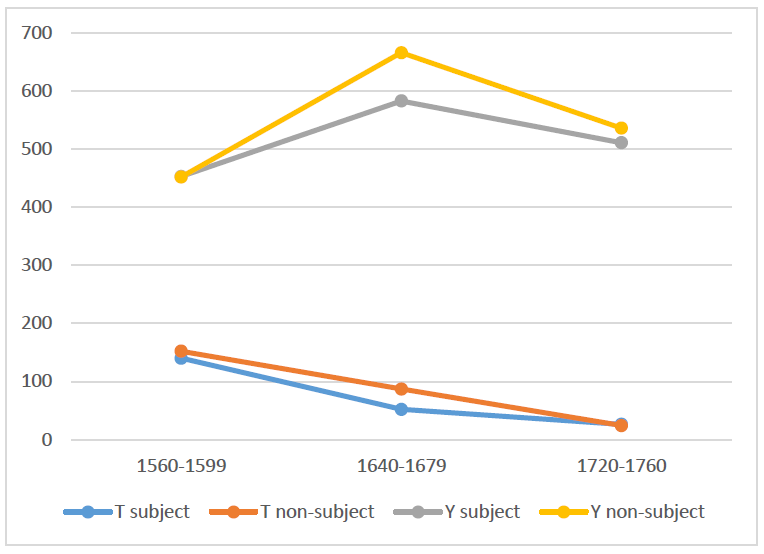
\includegraphics[width=.8\textwidth]{figures/dramcom.png}
\begin{tikzpicture}
  \begin{axis}[
    ybar,
    ymin=0,
    xtick=data,
    symbolic x coords={1560--1599, 1640--1679, 1720--1760},
    enlarge x limits=0.25,
    axis lines*=left,
    every axis plot/.append style={fill},
    cycle list name=Dark2-4,
    legend pos=outer north east,
    legend style={cells={anchor=west, font=\small}}
  ]
  \addplot coordinates {(1560--1599, 140) (1640--1679, 52) (1720--1760, 26)};
  \addplot coordinates {(1560--1599, 152) (1640--1679, 87) (1720--1760, 24)};
  \addplot coordinates {(1560--1599, 453) (1640--1679, 583) (1720--1760, 511)};
  \addplot coordinates {(1560--1599, 452) (1640--1679, 666) (1720--1760, 536)};
  \legend{T subject, T non-subject, Y subject, Y non-subject}
  \end{axis}
\end{tikzpicture}
\caption{T and Y subjects and non-subjects in drama comedy \citep[based on][320]{Walker2007}.\label{fig1}}
\end{figure}

In the comedies investigated by \citet{Walker2007}, overall, all forms of T decrease from 1560 to 1760, with the share of subjects and non-subjects \footnote{This category, actually labelled \enquote{subjective} in \citet{Walker2007}, overwhelmingly consists of pronouns in subject function. However, it also subsumes appositions, subject complements, and vocatives. The classification therefore is not perfect for our purpose, because ideally we would  compare the forms in subject function (i.e. those that trigger inflection on the verb) with all the others. According to \citet[260]{Walker2007}, though, the vast majority of the \enquote{subjective} forms are subjects anyway, so even if the few vocatives etc. were assigned to the non-subject category, the overall picture would probably not change greatly.}  (these include objects as well as possessive pronouns and determiners) being roughly equal in the first and the third subperiod (\tabref{tab8elsweiler} and \figref{fig1}). However, the reduction in T subjects is slightly stronger than in T non-subjects between the first two subperiods. Viewed in isolation, this could lend support to Aalberse \& Stoop’s (2015) claim. Yet the fact that in the same subperiod also in the Y forms, subjects are less numerous than non-subjects, again casts doubt on this interpretation. The overall lower share of subjects in address pronouns in this subperiod might have a different reason.

\begin{table}
\caption{T and Y in subjects and non-subjects in English trial proceedings, 16th–18th c.  \citep[321]{Walker2007}}
\label{tab9elsweiler}
\fittable{%
 \begin{tabular}{ll *{5}{r@{\,}r}} 
  \lsptoprule
     &				& \multicolumn{2}{c}{1560--1599} & \multicolumn{2}{c}{1600--1639} & \multicolumn{2}{c}{1640--1679} & \multicolumn{2}{c}{1680--1719} & \multicolumn{2}{c}{1720--1760}\\ 
  \midrule
  T  & subject 		&  80 & (65\%) &  10 & (59\%) &   6 &  (38\%) &   6 &  (50\%) & 0  & \\
     & non-subject  &  43 & (35\%) &   7 & (41\%) &  10 &  (63\%) &   6 &  (50\%) & 0  & \\
     & total    	& 123 &		   &  17 &		  &  16 &  	      &  12 &  		  & 0  & \\
  Y  & subject  	& 233 & (55\%) & 106 & (55\%) & 326 &  (72\%) & 435 &  (68\%) & 201& (64\%)  \\
     & non-subject  & 189 & (45\%) &  88 & (45\%) & 125 &  (28\%) & 204 &  (32\%) & 112& (36\%)  \\
     & total    	& 422 &		   & 194 &		  & 451 & 	      & 639 & 		  & 313&   \\
  \lspbottomrule
 \end{tabular} }
\end{table}
\il{English}

\begin{figure}
% % 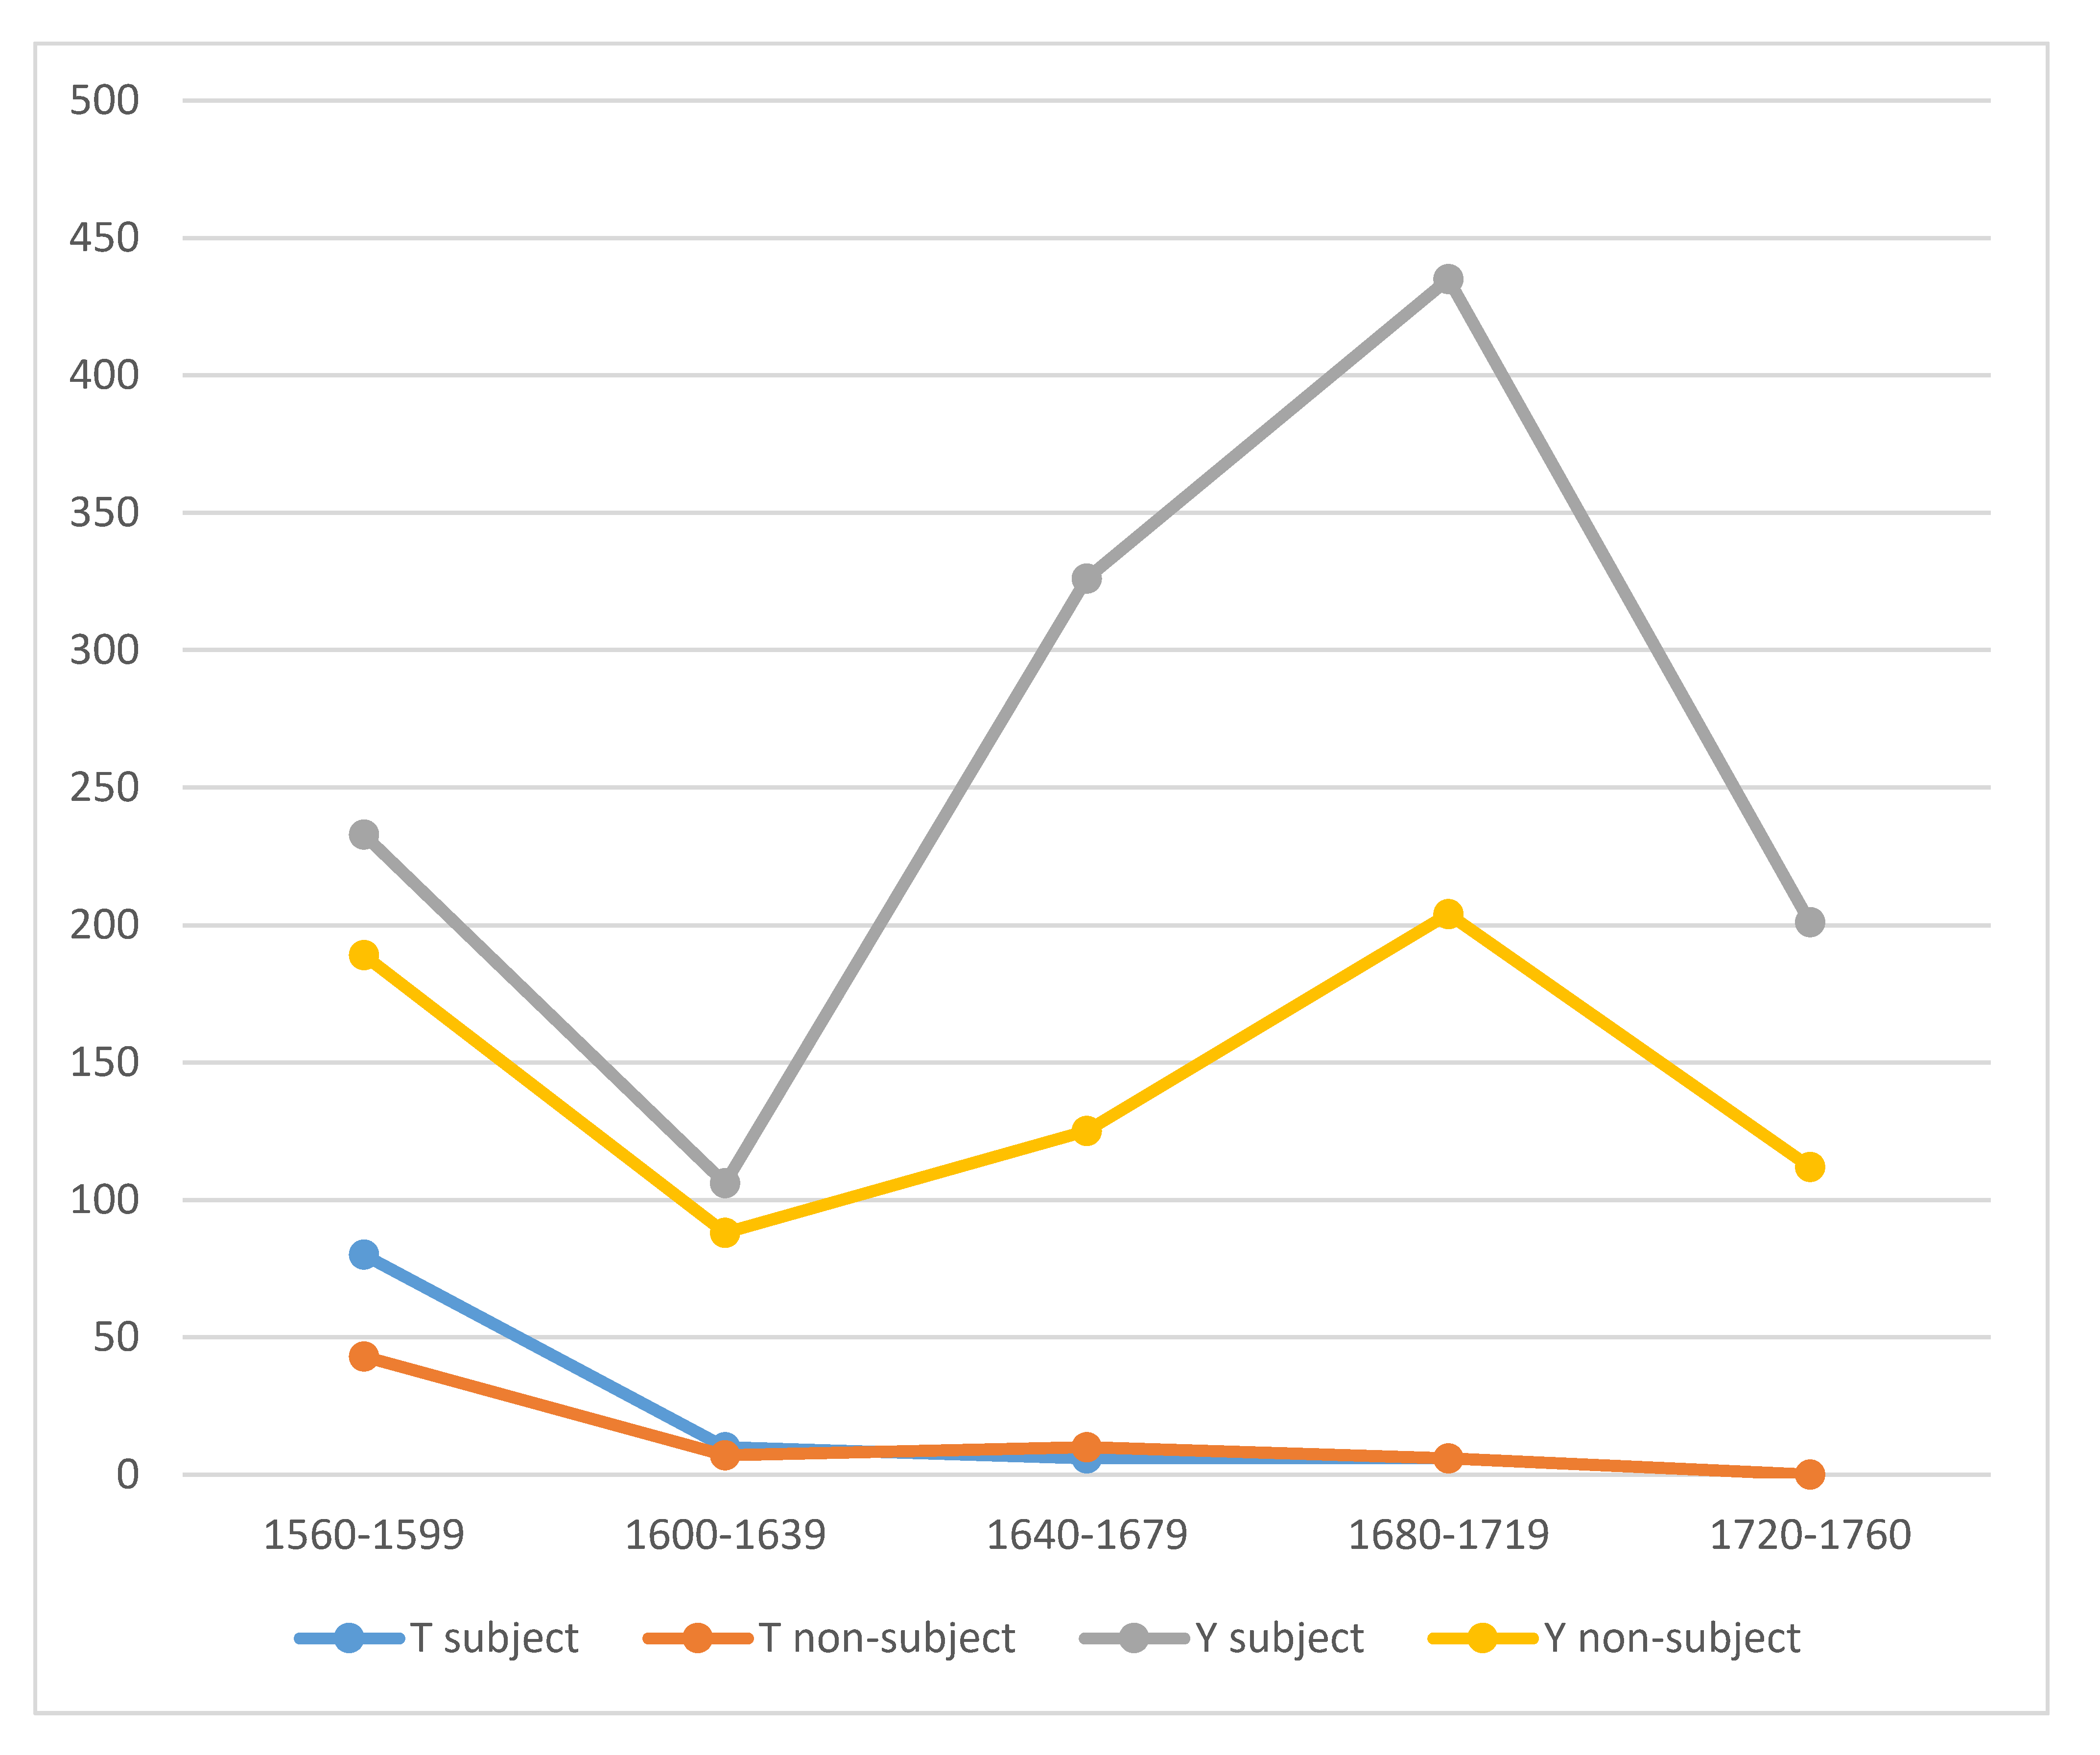
\includegraphics[width=.8\textwidth]{figures/tripro.png}
\begin{tikzpicture}
  \begin{axis}[
    width=\textwidth,
    height=7cm,
    ybar,
    ymin=0,
    xtick=data,
    symbolic x coords={1560--1599, 1600--1639, 1640--1679, 1680--1719, 1720--1760},
    enlarge x limits=0.15,
    axis lines*=left,
    every axis plot/.append style={fill},
    cycle list name=Dark2-4,
%     legend pos=outer north east,
    legend style={cells={anchor=west, font=\small}}
  ]
  \addplot coordinates {(1560--1599, 80) (1600--1639, 10) (1640--1679, 6) (1680--1719, 6) (1720--1760, 0)};
  \addplot coordinates {(1560--1599, 43) (1600--1639, 7) (1640--1679,10) (1680--1719, 6) (1720--1760, 0)};
  \addplot coordinates {(1560--1599, 233) (1600--1639, 106) (1640--1679, 326) (1680--1719, 435) (1720--1760, 201)};
  \addplot coordinates {(1560--1599, 189) (1600--1639, 88) (1640--1679, 125) (1680--1719, 204) (1720--1760, 112)};
  \legend{T subject, T non-subject, Y subject, Y non-subject}
  \end{axis}
\end{tikzpicture}
\caption{T and Y in subjects and non-subjects in trial proceedings \citep[based on][321]{Walker2007}.\label{fig2}}
\end{figure}

In the results from the trial proceedings (\tabref{tab9elsweiler} and \figref{fig2}), the initial decline of T is steeper in the subjects than in the non-subjects too, and in the third subperiod, subjects even become less numerous than non-subjects. However, the overall numbers of T are fairly low (between 17 and 0) after the first subperiod. Different from what we saw in the data from drama comedy, the share of subjects and non-subjects in the Y forms does not mirror the development in T; Y subjects remain more frequent than the other forms throughout. So the results could be cautiously taken to be in accordance with Aalberse \& Stoop’s hypothesis that speakers tend to avoid subject T more than other T forms. 

To conclude, the data found in the literature definitely do not yield a clear picture, but to some extent might support the scenario sketched by \citet{Aalberse2015}. \citet{Huberinprep} will examine it more closely by studying pronoun use in \ili{Early Modern English} letters as well as looking into the details of the contact situation in contemporary London.

\section{Conclusion}\label{sec:eh:6}

This paper has focused on the loss of the number contrast in the \ili{Standard English} 2nd person pronouns. This loss is undeniably a \enquote{change for the worse} for speakers, as attested to by the various repair strategies in different varieties of \ili{English} that we discussed in \sectref{sec:eh:2}. Yet, can the loss of number as a change for the worse be attributed to some \enquote{change for the better} in another area? We suggest that two changes for the better may have been involved here.

With the introduction and spread of the polite plural in \ili{Middle English}, as outlined in \sectref{sec:eh:3}, speakers could choose between two different sets of pronouns for singular address. This can be characterized as a sociopragmatic change for the better, since it constituted an addition to the pragmatic toolkit, a new means of sociopragmatic distinction. As we discussed in \sectref{sec:eh:4}, some speakers exploited the T/Y opposition for nuanced pragmatic differentiations. T was increasingly avoided though, and by the eighteenth century, Y had become the generally accepted unmarked standard form. Speakers avoided T because of its increasing stigmatization – a change from above in the Labovian sense. 

Yet the avoidance of T, we argue with \citet{Aalberse2015} in \sectref{sec:eh:5}, may have been additionally driven by a change from below: the avoidance of the inflectional ending \{-\textit{st}\} that comes along with T. Getting rid of \{-\textit{st}\} results in a much simplified verbal paradigm, which clearly represents a structural \enquote{change for the better}, particularly in the linguistic situation of early modern London, with many second language and second dialect learners. In the literature on \ili{English}, this has hitherto not been taken into consideration; on the contrary, the \enquote{fate of the 2s inflection} is usually depicted as being doomed to die with the pronoun \textit{thou} \citep[e.g.][162]{Lass1999}. We suggest that this might have been more of a bilateral story: Rather than a mere casualty, \{-\textit{st}\} may have been one of the responsible factors in the loss of T. The trajectories of T-loss in subjects and non-subjects in texts from the early modern period that we presented in \sectref{sec:eh:5} can cautiously be taken as initial support for the idea that deflection may be one of the driving forces in the loss of T in \ili{English}, but clearly more research is needed. 


\nocite{CEEC} \nocite{OED}
\printbibliography[heading=subbibliography,notkeyword=this]

\end{document}

% Interne Anmerkungen und Fragen:
%
% Wird "second" ausgeschrieben?
%
% "y'all" vs "yall": Ist im Original gemischt.
%
% Mazzon2010 & Wright1997 fehlt im .bib-file 
